%%%%%%%%%%%%%%%%%%%%%%%%%%%%%%%%%%%%%%%%%%%%%%%%%%%%%%%%%%%%%%%%%%%%
% Medical Data and imaging
%%%%%%%%%%%%%%%%%%%%%%%%%%%%%%%%%%%%%%%%%%%%%%%%%%%%%%%%%%%%%%%%%%%%
%!TeX spellcheck = en-GB
\chapter{Medical Data and imaging}
  \label{Medical Data and imaging}
\section{DICOM Format}
\begin{wrapfigure}{r}{0.3\textwidth}
    \vspace{-10pt}
   \centering
   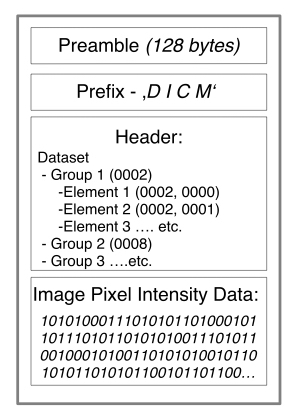
\includegraphics[width=0.28\textwidth]{figures/dicom.jpeg}
    \caption{structure of a DICOM file }
    \label{figure 2.1}
    \vspace{-15pt}
\end{wrapfigure}
DICOM  stands for Digital Imaging and Communications in Medicin. It provides standardized file format for images in medicine. Each DICOM file is made up of a header holding meta data and a body which contains the image. DICOM files tend to be fairly large, as they usually contain quite a few high resolution images. The meta data consists of a standardized series of tags which can be arranged in functional groups like "0010" patient information or "0008" study information.
DICOM images that are used for research or teaching are typically anonymized to protect the patients data. There are special programms to remove the according parts from the header.
Since DICOM files are not recognized as image files by most operating systems, including windows, macOS and ubuntu, they can only be viewed with the help of third-party software.
Thats why most equipment manufacturers either include a dicom viewer when the images are exported to a CD or just convert them to a JPEG, GIF or TIFF.
\cite{varmaManagingDICOMImages2012}
 \cite{ElsevierEnhancedReader}

  \section{Image Aquisition}
 \label{Image Aquisition}
 There are many different types of medical imaging. Each method has their own purpose and often more than one type of image is required to make a correct diagnosis. The first most common and also foundation for all other type of imaging techniques being an X-ray scan. It is on of the fastest methods to check for a bone fracture or tooth decay. However,  an X-ray don't have a depth of field therefore only show one view through the patients body. Hence sometimes an important detail can't be seen because it lies behind a less permeable material. PET Scans, CTs and MRI Scans give us the option to image the whole volume or a planar slice thorugh it. In the following I will give a quick summary on 2d, 3d and 4d datasets using the MRI scanning methodology as an example.

 \subsection{2d Slices}
  \label{2d Slice}
 In an MRI scanner a magnetic field is created, so that all protons in the patients body align themselfs with that field.
A 2d image is created by exciting a slice of tissue with a radio frequency (RF) impulse so that the protons in said tissue spin out of equilibrium.  and then detect the energy released when the protons in the tissue realign with the magnetic field.
\cite{MagneticResonanceImaging}
The thickness of the slices depend on the device used, but are normally between 2mm and 100mm.
\cite{johnson2DMultislice3D1999}
Modern machines are able to excite multiple slices of tissue, therefore making it possible to scan multiple slices at a time. This technique is called a 2D Multislice MRI.
\cite{vangeunsBasicPrinciplesMagnetic1999}

  \subsection{3d Volumetric imaging}
  \label{3d Volumetric imaging}
  There are two main ways to get a 3d image. One of these being a reconstruction of the original volume thorugh a collection of 2d slices. This sounds very simple, but there are actually may things to consider. Firstly, scantimes can be quite long, as there needs to be a short pause inbetween scans. Pictures need to be taken in the exact same position to avoid artifacts. Furthermore there will always be a space inbetween two slices. With methods such as the distance field interpolation, we have tools to overcome this proplem to a certain extent, but it will never be as exact as the second method of 3d imaging.
  \cite{vangeunsBasicPrinciplesMagnetic1999}
  Here, a whole slab of the volume gets excited.


  \subsection{4d medical imaging}
  \label{4d medical imaging}
  4d medical imaging is the process of generating multiple 3d images over time. It is an advanced imaging method, used to study a patients movements and observe changes. The human body naturally moves at all times. Respiratory and cardiac motion, as well as digestion and muscle movements, cause the movement of surrounding tissues. It has always been a challenge to capture these movements in 3d medical images or get an image in a good position to see a certain feature. With 4d imaging, medical professionals are able to capture the whole movement and pick the best time frames for their issue.

\section{Image-guided therapy}
\label{Image-guided therapy}

\subsection{planning}
  \label{planning}
When planning an operation or radiation session, MRI is mainly used for gross tumor volume (GTV) and organs at risk (OAR) delineation.
\cite{lineyMRIRadiotherapyPlanning2019}

  \subsection{radiotherapy and LINAC}
    \label{radiotherapy and LINAC}
stereotactic radiosurgery (SRS)
